

\tikzset{every picture/.style={line width=0.75pt}} %set default line width to 0.75pt        

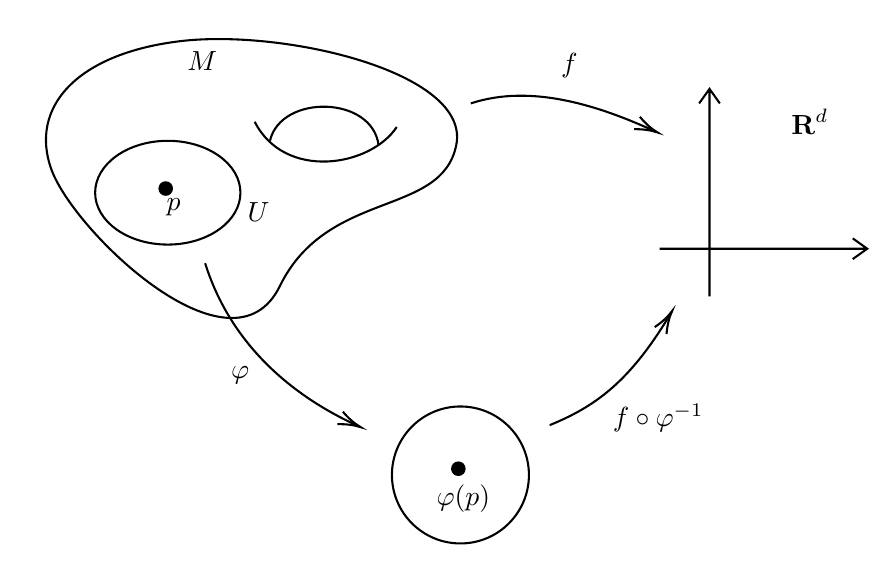
\begin{tikzpicture}[x=0.75pt,y=0.75pt,yscale=-1,xscale=1]
%uncomment if require: \path (0,436); %set diagram left start at 0, and has height of 436

%Shape: Polygon Curved [id:ds8701230940513227] 
\draw   (188,45) .. controls (238,39) and (328,60) .. (321,95) .. controls (314,130) and (259,116) .. (236,163) .. controls (213,210) and (137,137) .. (126,107) .. controls (115,77) and (138,51) .. (188,45) -- cycle ;
%Curve Lines [id:da00033147629047403093] 
\draw    (223.88,83.82) .. controls (238.3,112.28) and (279.62,105.58) .. (292.31,86.36) ;
%Curve Lines [id:da9461703131021257] 
\draw    (231.26,92.91) .. controls (236.56,70.44) and (280.47,71.1) .. (283.57,95.11) ;
%Shape: Ellipse [id:dp5760164398280032] 
\draw   (147,118) .. controls (147,104.19) and (162.67,93) .. (182,93) .. controls (201.33,93) and (217,104.19) .. (217,118) .. controls (217,131.81) and (201.33,143) .. (182,143) .. controls (162.67,143) and (147,131.81) .. (147,118) -- cycle ;
%Shape: Circle [id:dp35830362116000813] 
\draw  [fill={rgb, 255:red, 0; green, 0; blue, 0 }  ,fill opacity=1 ] (178,116) .. controls (178,114.34) and (179.34,113) .. (181,113) .. controls (182.66,113) and (184,114.34) .. (184,116) .. controls (184,117.66) and (182.66,119) .. (181,119) .. controls (179.34,119) and (178,117.66) .. (178,116) -- cycle ;

%Shape: Axis 2D [id:dp28763923911889777] 
\draw  (419,145) -- (519,145)(443,68) -- (443,168) (512,140) -- (519,145) -- (512,150) (438,75) -- (443,68) -- (448,75)  ;
%Shape: Circle [id:dp46748884211924646] 
\draw   (290,254) .. controls (290,235.77) and (304.77,221) .. (323,221) .. controls (341.23,221) and (356,235.77) .. (356,254) .. controls (356,272.23) and (341.23,287) .. (323,287) .. controls (304.77,287) and (290,272.23) .. (290,254) -- cycle ;
%Curve Lines [id:da19106736276909064] 
\draw    (200,152) .. controls (210.84,186.48) and (236.22,213.19) .. (273.3,230.23) ;
\draw [shift={(275,231)}, rotate = 204.1] [color={rgb, 255:red, 0; green, 0; blue, 0 }  ][line width=0.75]    (10.93,-3.29) .. controls (6.95,-1.4) and (3.31,-0.3) .. (0,0) .. controls (3.31,0.3) and (6.95,1.4) .. (10.93,3.29)   ;
%Shape: Circle [id:dp4052608591994611] 
\draw  [fill={rgb, 255:red, 0; green, 0; blue, 0 }  ,fill opacity=1 ] (319,251) .. controls (319,249.34) and (320.34,248) .. (322,248) .. controls (323.66,248) and (325,249.34) .. (325,251) .. controls (325,252.66) and (323.66,254) .. (322,254) .. controls (320.34,254) and (319,252.66) .. (319,251) -- cycle ;
%Curve Lines [id:da5944217136756031] 
\draw    (328,75) .. controls (357.4,65.2) and (390.64,76.53) .. (416.43,88.28) ;
\draw [shift={(418,89)}, rotate = 204.78] [color={rgb, 255:red, 0; green, 0; blue, 0 }  ][line width=0.75]    (10.93,-3.29) .. controls (6.95,-1.4) and (3.31,-0.3) .. (0,0) .. controls (3.31,0.3) and (6.95,1.4) .. (10.93,3.29)   ;
%Curve Lines [id:da8968041677982646] 
\draw    (366,230) .. controls (387.67,221.14) and (404.49,209.36) .. (424.1,176.52) ;
\draw [shift={(425,175)}, rotate = 120.47] [color={rgb, 255:red, 0; green, 0; blue, 0 }  ][line width=0.75]    (10.93,-3.29) .. controls (6.95,-1.4) and (3.31,-0.3) .. (0,0) .. controls (3.31,0.3) and (6.95,1.4) .. (10.93,3.29)   ;

% Text Node
\draw (180,119.4) node [anchor=north west][inner sep=0.75pt]    {$p$};
% Text Node
\draw (190,48.4) node [anchor=north west][inner sep=0.75pt]    {$M$};
% Text Node
\draw (219,121.4) node [anchor=north west][inner sep=0.75pt]    {$U$};
% Text Node
\draw (211,200.4) node [anchor=north west][inner sep=0.75pt]    {$\varphi $};
% Text Node
\draw (310,257.4) node [anchor=north west][inner sep=0.75pt]    {$\varphi ( p)$};
% Text Node
\draw (370,49.4) node [anchor=north west][inner sep=0.75pt]    {$f$};
% Text Node
\draw (395,218.4) node [anchor=north west][inner sep=0.75pt]    {$f\circ \varphi ^{-1}$};
% Text Node
\draw (481,76.4) node [anchor=north west][inner sep=0.75pt]    {${\displaystyle \mathbf{R}^{d}}$};


\end{tikzpicture}
